\documentclass{standalone}

\usepackage{tikz}
\usetikzlibrary{calc}
\usetikzlibrary{math}

\begin{document}

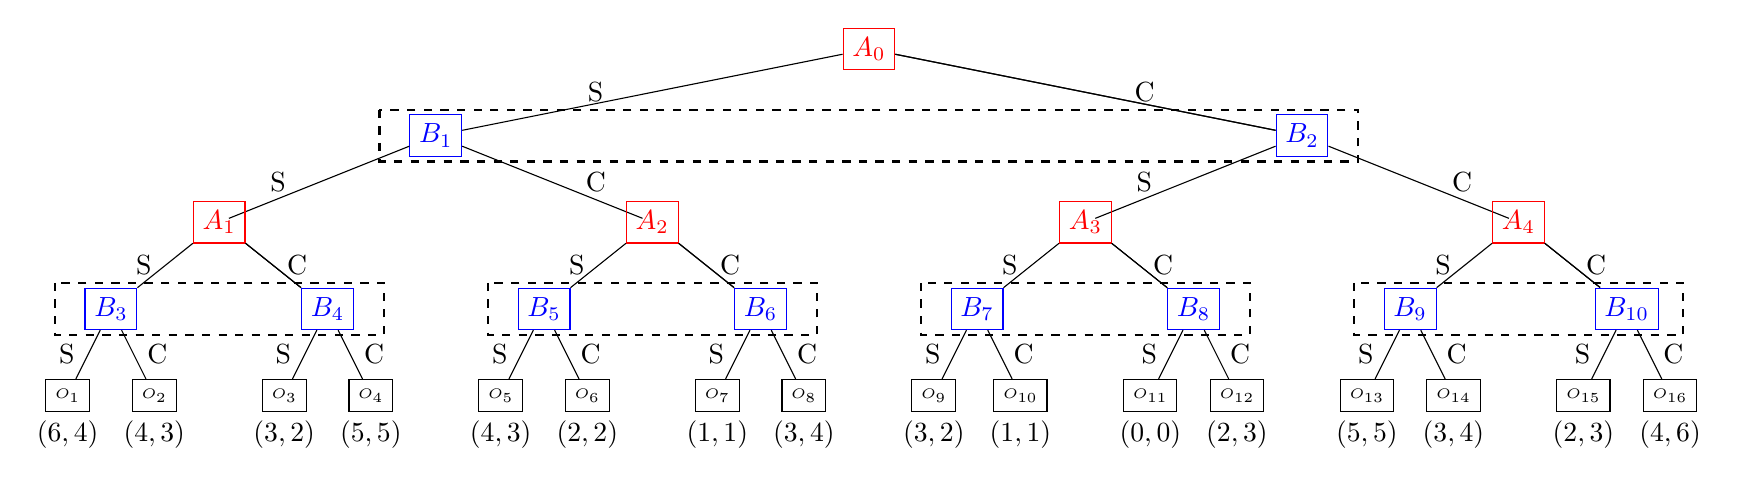
\begin{tikzpicture}

    \tikzset{stagegame/.pic={
    \node [draw, color=red] (A) at (0, 0) {\(A_0\)};
        \node [draw, color=blue] (B1) at ($(A) + (-5, -1)$) {\(B_1\)};
            \node (O1) at ($(B1) + (-2.5, -1)$) {};
            \node (SS) at ($(O1) + (0, -.5)$) {};
            \node (O2) at ($(B1) + (2.5, -1)$) {};
            \node (SC) at ($(O2) + (0, -.5)$) {};
        \node [draw, color=blue] (B2) at ($(A) + (5, -1)$) {\(B_2\)};
            \node (O3) at ($(B2) + (-2.5, -1)$) {};
            \node (CS) at ($(O3) + (0, -.5)$) {};
            \node (O4) at ($(B2) + (2.5, -1)$) {};
            \node (CC) at ($(O4) + (0, -.5)$) {};
    \draw (A) -- node[left=5mm, midway] {S} (B1);
    \draw (A) -- node[right=5mm, midway] {C} (B2);
        \draw (B1)  -- node[left=3mm, midway] {S}  (O1);
        \draw (B1) -- node[right=3mm, midway] {C} (O2);
    \draw (A) -- (B2);
        \draw (B2)  -- node[left=3mm, midway] {S}  (O3);
        \draw (B2) -- node[right=3mm, midway] {C} (O4);

    \draw  [dashed, thick] ($(B1) + (-.65, .3)$) rectangle  ($(B2) + (.65, -.3)$);
        }
    }
    \pic[scale=1.1]{stagegame};

    \tikzset{repeatedstagegame/.pic={
        \tikzmath{\x1 = int(2 * #1 + 1);}
        \tikzmath{\x2 = int(\x1 + 1);}
        \tikzmath{\z1 = int(1 + 4 * (#1 - 1));}
        \tikzmath{\z2 = int(\z1 + 1);}
        \tikzmath{\z3 = int(\z2 + 1);}
        \tikzmath{\z4 = int(\z3 + 1);}

        \node [draw, color=red] (A) at (0, 0) {\(A_{#1}\)};
        \node [draw, color=blue] (B1) at ($(A) + (-1.25, -1)$) {\(B_{\x1}\)} ;
        \node [draw] (O1) at ($(B1) + (-.5, -1)$) {\tiny{\(O_{\z1}\)}};
        \node [draw] (O2) at ($(B1) + (.5, -1)$) {\tiny{\(O_{\z2}\)}};
        \node [draw, color=blue] (B2) at ($(A) + (1.25, -1)$) {\(B_{\x2}\)};
        \node [draw] (O3) at ($(B2) + (-.5, -1)$) {\tiny{\(O_{\z3}\)}};
        \node [draw] (O4) at ($(B2) + (.5, -1)$) {\tiny{\(O_{\z4}\)}};
        \draw (A) -- node[left=.5mm, midway] {S} (B1);
        \draw (A) -- node[right=.5mm, midway] {C} (B2);
        \draw (B1)  -- node[left=.5mm, midway] {S}  (O1);
        \draw (B1) -- node[right=.5mm, midway] {C} (O2);
        \draw (A) -- (B2);
        \draw (B2)  -- node[left=.5mm, midway] {S}  (O3);
        \draw (B2) -- node[right=.5mm, midway] {C} (O4);

        \draw  [dashed, thick] ($(B1) + (-.65, .3)$) rectangle  ($(B2) + (.65, -.3)$);
    }
    }
    \pic at (O1) [scale=1.1]{repeatedstagegame={1}};
        \node at ($(O1) + (0, -.5)$) {\((6, 4)\)};
        \node at ($(O2) + (0, -.5)$) {\((4, 3)\)};
        \node at ($(O3) + (0, -.5)$) {\((3, 2)\)};
        \node at ($(O4) + (0, -.5)$) {\((5, 5)\)};
    \pic at ($(A) + (5.5, 0)$) [scale=1.1]{repeatedstagegame={2}};
        \node at ($(O1) + (0, -.5)$) {\((4, 3)\)};
        \node at ($(O2) + (0, -.5)$) {\((2, 2)\)};
        \node at ($(O3) + (0, -.5)$) {\((1, 1)\)};
        \node at ($(O4) + (0, -.5)$) {\((3, 4)\)};
    \pic at ($(A) + (5.5, 0)$) [scale=1.1]{repeatedstagegame={3}};
        \node at ($(O1) + (0, -.5)$) {\((3, 2)\)};
        \node at ($(O2) + (0, -.5)$) {\((1, 1)\)};
        \node at ($(O3) + (0, -.5)$) {\((0, 0)\)};
        \node at ($(O4) + (0, -.5)$) {\((2, 3)\)};
    \pic at ($(A) + (5.5, 0)$) [scale=1.1]{repeatedstagegame={4}};
        \node at ($(O1) + (0, -.5)$) {\((5, 5)\)};
        \node at ($(O2) + (0, -.5)$) {\((3, 4)\)};
        \node at ($(O3) + (0, -.5)$) {\((2, 3)\)};
        \node at ($(O4) + (0, -.5)$) {\((4, 6)\)};

\end{tikzpicture}

\end{document}
